\documentclass[a4paper,11pt,fleqn]{article}%fleqn pour aligner les equations à gauche
\usepackage{../../Styles/Cours}

\newcommand{\chnum}{Chapitre 17}
\newcommand{\chtitle}{Découverte de l'effet Doppler}
\newcommand{\dtype}{Activité}

\begin{document}
\maketitle

En 1942, le physicien autrichien Christian Doppler modélise un phénomène caractéristique des ondes émises par des sources en mouvement, et le présente à l'Académie royale des sciences de Bohème. En 1845, le physicien autrichien Christoph Buys-Ballot réalise une expérience pour tester la théorie de Doppler.

\vspace{1em}

\noindent\fbox{\begin{minipage}{.5\linewidth}
\textbf{Document 1 : Abaissement du ton au passage d'un train}\\
\begin{center}
    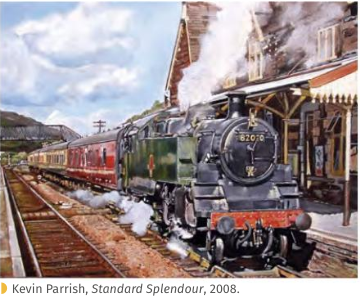
\includegraphics[scale=.6]{Ressources/TSPE_C17_Act_Fig0.png}
\end{center}
On peut observer, à chaque station de chemin de fer, un effet de ce genre extrêmement instructif, au moment du passage d'un train à grande vitesse. Pendant qu'il approche, les ondes émises par le sifflet sont virtuellement ou équivalemment raccourcies, parce qu'il en arrive un plus grand nombre à l'oreille, dans un temps donné.\\
Quand il s'éloigne au contraire, les ondes sonores sont virtuellement ou équivalement rendues plus longues. La conséquence de ce raccourcissement et de cet allongement est que, lorsque le train d'approche, le sifflet rend un son plus aigu et lorsqu'il s'éloigne, le sifflet rend un son plus grave que lorsque le train est au repos.\\
On perçoit donc à chaque passage du train un abaissement du ton. Des expériences de ce genre ont été faites sur les chemins de fer hollandais par M. Buys-Ballot, et plus tard en Angleterre par M. Scott-Russel.
\end{minipage}}
\begin{minipage}{.48\linewidth}
    \fbox{\begin{minipage}{\linewidth}
    \textbf{Document 2 : Expérience de Buys-Ballot}
    \begin{center}
        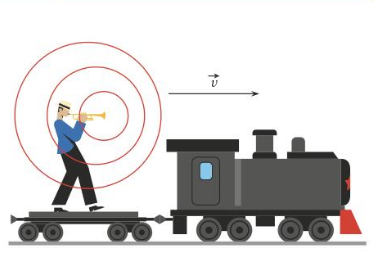
\includegraphics[scale=.4]{Ressources/TSPE_C17_Act_Fig1.png}
    \end{center}
    Le 3 juin 1845, afin de tester les théories de Christan Doppler, Christoph Buys-Ballot place des musiciens sur un train et leur demande de jouer un \emph{la$_3$}.\\
    Il place sur le quai, à des intervalles réguliers, des groupes d'autres musiciens capables de distinguer très finement les différences de hauteur de notes. Lorsque le train s'est approché, les musiciens restés à quai ont affirmé avoir entendu un \emph{si$b_3$}, soit une note plus aiguë d'un demi-ton.
    \end{minipage}}
    \fbox{\begin{minipage}{\linewidth}
    \textbf{Document 3 : L'effet Doppler}\\
    Lorsqu'un émetteur d'onde est en mouvement à une vitesse $v$ par rapport à un récepteur fixe, la fréquence $f_{rec}$ reçue par le récepteur diffère de la fréquence $f_{em}$ émise selon les formules suivantes :
    \begin{itemize}
        \item Si l'émetteur et le récepteur se rapprochent : $$f_{rec}=\dfrac{f_{em}\cdot v_{onde}}{v_{onde}-v}$$
        \item Si l'émetteur et le récepteur s'éloignent : $$f_{rec}=\dfrac{f_{em}\cdot v_{onde}}{v_{onde}+v}$$
    \end{itemize}
    \end{minipage}}
    \end{minipage}


\noindent\fbox{\begin{minipage}{\linewidth}
\textbf{Document 4 : Source sonore en mouvement}\\
\begin{center}
    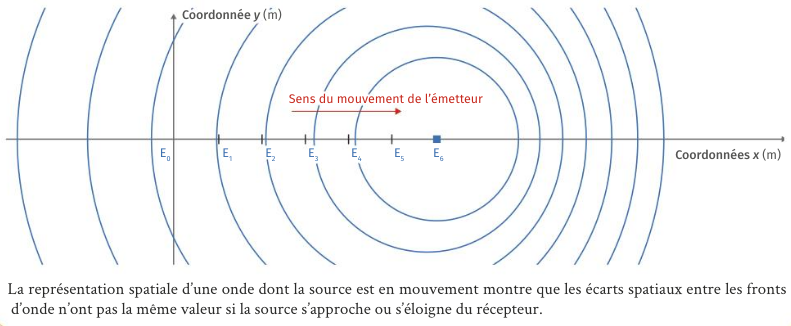
\includegraphics[scale=.5]{Ressources/TSPE_C17_Act_Fig2.png}
\end{center}
\end{minipage}}

\noindent\fbox{\begin{minipage}{\linewidth}
\textbf{Document 5 : Fréquences de quelques notes de musiques}\\
\begin{tabular}{|>{\centering}m{2cm}|c|c|c|c|c|c|c|}
    \hline \textbf{Note} & \emph{sol$_3$}& \emph{sol\#$_3$}& \emph{la$_3$}& \emph{si$b_3$}& \emph{si$_3$}& \emph{do$_4$}& \emph{do\#$_4$}\\
    \hline \textbf{Fréquence (\unit{\hertz})}& 392 & 415 & 440 & 466 & 494 & 523 & 554\\
    \hline
\end{tabular}

\textbf{Données : }
\begin{itemize}
    \item \textbf{Vitesse du son dans l'air :} $v_{son}$ = \SI{340}{\meter\per\second}
    \item \textbf{Célérité de la lumière dans le vide :} $c$ = \SI{3,00E8}{\meter\per\second}
\end{itemize}
\end{minipage}}

\vspace{.5cm}
\textbf{Questions : }
\begin{enumerate}
    \item \begin{enumerate}
        \item Exprimer la longueur d'onde de l'onde reçue $\lambda_{rec}$ par l'observateur en fonction de $f_{rec}$ et $v_{onde}$ dans le référentiel terrestre.
        \item Exprimer les vitesses $v_1$ et $v_2$ de l'onde dans le référentiel lié à l'émetteur, en fonction de $v_{onde}$ et $v$, respectivement dans le cas d'un éloignement et d'un rapprochement entre l'émetteur et le récepteur.
        \item En déduire une expression des longueurs d'onde $\lambda_1$ et $\lambda_2$ (respectivement dans le cas d'un éloignement et d'un rapprochement) de l'onde émise dans le référentiel de l'émetteur en fonction de $f_{em}$, $v_{onde}$ et $v$.
        \item  En décrivant l'égalité entre les longueurs d'onde exprimées dans les deux référentiels, retrouver les formules données dans le Document 3.
    \end{enumerate}
    \item Expliquer pourquoi les musiciens restés à quai ont entendu une note plus aiguë que celle jouée sur le train.
    \item Calculer al vitesse à laquelle ce train se déplaçait.
    \item En déduire la note entendue par les musiciens à quai lorsque le train s'éloignait.
    \item Calculer la vitesse que le train devrait avoir pour que les musiciens entendent un \emph{do$_4$}. Commenter.
\end{enumerate}

\end{document}

